% -*- TeX-engine: luatex -*-
\documentclass[presentation,aspectratio=43,10pt]{beamer}
\usepackage{pgfplots}
\pgfplotsset{compat=1.15}
\usepackage{template}
\renewcommand{\authorname}{Lawrence Mitchell\inst{*}}
\renewcommand{\authoremail}{\inst{*}\texttt{lawrence.mitchell@durham.ac.uk}}

\renewcommand{\sessionnumber}{7}
\renewcommand{\sessiontitle}{Vectorisation and data layout}
\usepackage{tikz}
\usetikzlibrary{matrix,fit,positioning,calc}
\usepackage{pgfplotstable}
\usepackage{booktabs}
\usetikzlibrary{pgfplots.groupplots}
\date{}

\begin{document}
\begin{frame}
  \maketitle
\end{frame}

\begin{frame}[fragile]
  \frametitle{Current status}
  
  \begin{answer}{So far}
    Only looked at simple data structures and loop nests
    
  $\Rightarrow$ Loop unrolling, tiling, and judicious alignment
    sufficient for vectorisation
\begin{minted}{c}
for (i = 0; i < N; i++)
  for (j = 0; j < K; j++)
    C[i] = f(a[i], b[j]);
\end{minted}
  \end{answer}

  \begin{challenge}{Question}
  What about \emph{more complicated} data structures or loops?
    
  $\Rightarrow$ Need to consider data layout transformations
  \emph{in tandem with} loop transformations
  \end{challenge}
\end{frame}

\begin{frame}[fragile]
  \frametitle{Motivating problems}
  \begin{challenge}{Stencil computations}
    7-point Laplacian
    \begin{equation*}
      B_{i,j,k} = A_{i-1,j,k} + A_{i,j-1,k} + A_{i,j,k-1} +
      A_{i+1,j,k} + A_{i,j+1,k} + A_{i,j,k+1} - 6 A_{i,j,k} \quad
      \forall i,j,k
    \end{equation*}
\begin{minted}[fontsize=\scriptsize]{c}
  for (int i = 1; i < n-1; i++)
    for (int j = 1; j < n-1; j++)
      for (int k = 1; k < n-1; k++)
        B[i, j, k] = (A[i-1, j, k] + A[i, j-1, k] + A[i, j, k-1]
                      + A[i+1, j, k] + A[i, j+1, k] + A[i, j, k+1]
                      - 6*A[i, j, k]);
\end{minted}
  \end{challenge}
  \begin{exampleblock}{Structs}
    Computation on 3D points
\begin{minted}[fontsize=\scriptsize]{c}
  struct point {
    double x, y, z;
  };
  for (int i = 0; i < n; i++) {
    l1dist[i] = fabs(points[i].x) + fabs(points[i].y) + fabs(points[i].z);
  }
\end{minted}
  \end{exampleblock}
\end{frame}

\begin{frame}
  \frametitle{Observations}
  \begin{itemize}
  \item Typical stencil loop has \emph{low} arithmetic intensity
  \item e.g.~five-point stencil does 5 flops on 5 doubles,
    for a computational intensity of $5 / (5*8) = 1/8$ FLOPs/byte.
  \item[$\Rightarrow$] Relevant machine limit is \emph{memory
      bandwidth}
  \item There is some data locality we can exploit, but not just
    stride-1 streams
  \item[$\Rightarrow$] tiling for locality is worthwhile
  \end{itemize}
\end{frame}

\begin{frame}[fragile]
  \frametitle{Complications}
  \begin{itemize}
  \item Typewriter (standard loop) iteration has low \emph{spatial
      locality}
  \item Have perfect access pattern for \texttt{[i, j]} indexing
  \item \texttt{[i+/-1, j]} indices miss cache every 8 updates (64
    byte cache lines, double precision), similar to matrix-transpose example.
  \item[$\Rightarrow$] loop tiling of \texttt{i} and \texttt{j} to
    promote cache reuse.
\begin{minted}[fontsize=\scriptsize]{c}
N = n / b; /* Tile with block size b */
for (ii = 0; ii < N; ii += b)
  for (jj = 0; jj < N; jj += b)
    for (i = ii; i < min(n, i + b); i++)
      for (j = jj; j < min(n, j + b); j++)
        b[i, j] = a[i-1,j] + a[i+1,j] + a[i,j-1] + a[i,j+1] - 4*a[i,j];
\end{minted}
  \item Still leaves us with problematic access patterns for
    vectorisation.
  \end{itemize}
\end{frame}

\begin{frame}
  \frametitle{Layer condition for tile size}
  Realistic worst case: 4 reads, 1 write per \emph{lattice update} (LUP) $\Rightarrow
    5 \cdot 8 = 40 \frac{\text{Byte}}{\text{LUP}}$.

    Best case: 2 reads, 1 write $\Rightarrow 3 \cdot 8 = 24\frac{\text{Byte}}{\text{LUP}}$.
  \begin{center}
    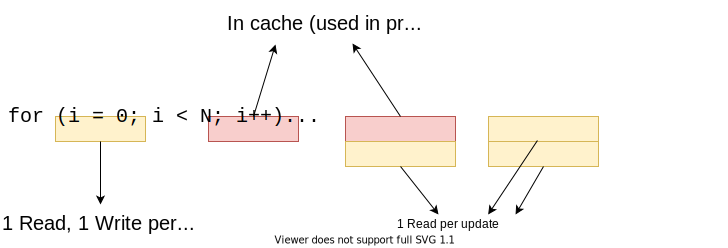
\includegraphics[height=0.5\textheight]{figures/stencilupdates}
  \end{center}
\end{frame}
\begin{frame}
  \frametitle{Picture}
  Worst case: cache \emph{not large enough} to hold three layers
  (rows) of grid.
  \begin{center}
    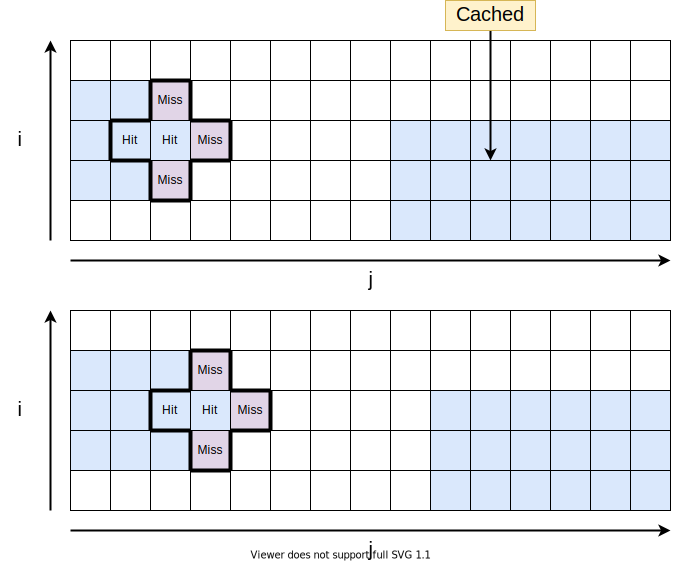
\includegraphics[height=0.7\textheight]{figures/layercondition}
  \end{center}
\end{frame}
\begin{frame}
  \frametitle{Layer condition solution}
  Tile inner loop dimension until layers fit in cache
  \begin{center}
    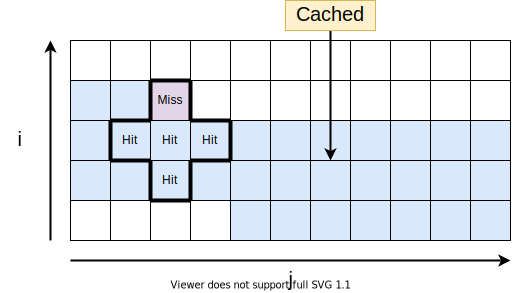
\includegraphics[height=0.35\textheight]{figures/layerconditiontiled}
  \end{center}
  \begin{answer}{Guideline}
    Choose blocking factor such that
    \begin{equation*}
      3 \cdot \text{block size} \cdot 8 \text{Bytes} <
      \text{CacheSize} / \underbrace{2}_{\text{Safety factor}}
    \end{equation*}
  \end{answer}
\end{frame}
\begin{frame}[fragile]
  \frametitle{Spatial blocking}
  \begin{challenge}{Before}
\begin{minted}{c}
  for (i = 0; i < imax; i++)
    for (j = 0; j < jmax; j++)
      y[i, j] = (x[i-1,j] + x[i+1,j] + x[i,j-1] 
                 + x[i,j+1] - 4*x[i,j]);
\end{minted}
  \end{challenge}
  \begin{answer}{After}
\begin{minted}{c}
  for (jb = 0; jb < jmax; jb += jblock)
    for (i = 0; i < imax; i++)
      for (j = jb; j < min(jb + jblock, jmax); j++)
        y[i, j] = (x[i-1,j] + x[i+1,j] + x[i,j-1] 
                   + x[i,j+1] - 4*x[i,j]);
\end{minted}
    \begin{equation*}
      \text{jblock} < \frac{\text{CacheSize}}{48 \text{Bytes}}
    \end{equation*}
  \end{answer}
\end{frame}
\begin{frame}
  \frametitle{Exercise}
  \begin{itemize}
  \item Measure performance of 5 point stencil. Can you determine when
    layer condition is not fulfilled. What does using tiling do to the
    performance?
  \item[$\Rightarrow$] Exercise 10.
  \end{itemize}
\end{frame}

\begin{frame}
  \frametitle{Loop reordering not enough}
  \begin{center}
    \only<1>{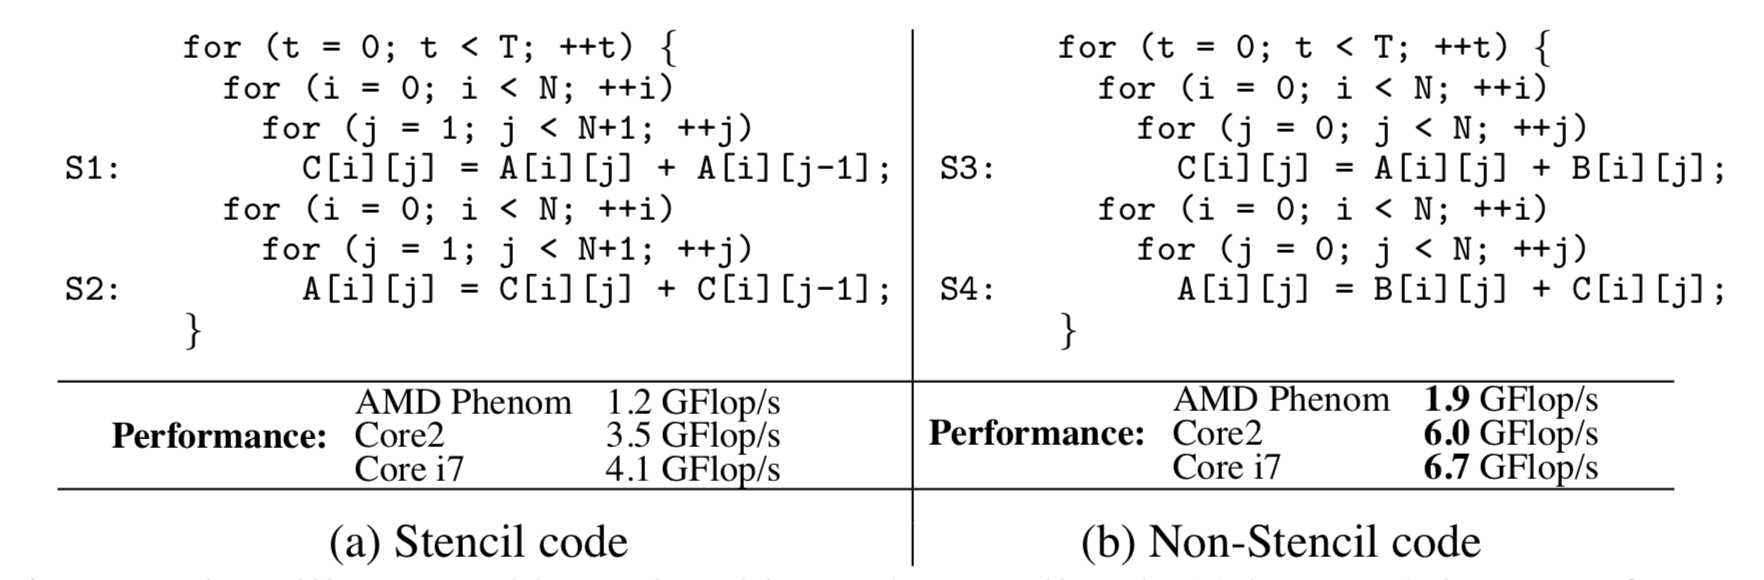
\includegraphics[width=\textwidth]{07/stencil-vs-nonstencil}}
    \only<2>{
  \begin{itemize}
  \item Vectorisation in inner loops $\Leftrightarrow$ operations on
    \emph{streams} of \emph{contiguous} data in memory.
  \item \texttt{C[i, j] = A[i, j] + B[i, j]} adds the stream of data
    \texttt{A[i, 1:N]} to another stream from \texttt{B[i, 1:N]}.
  \item In contrast \texttt{C[i, j] = A[i, j] + A[i, j-1]} adds
    \texttt{A[i, 1:N]} and \texttt{A[i, 0:N-1]}.
  \item These shifted streams necessitate inter-register shuffles (or
    explicit load/store operations).
  \end{itemize}
}      
    \only<3>{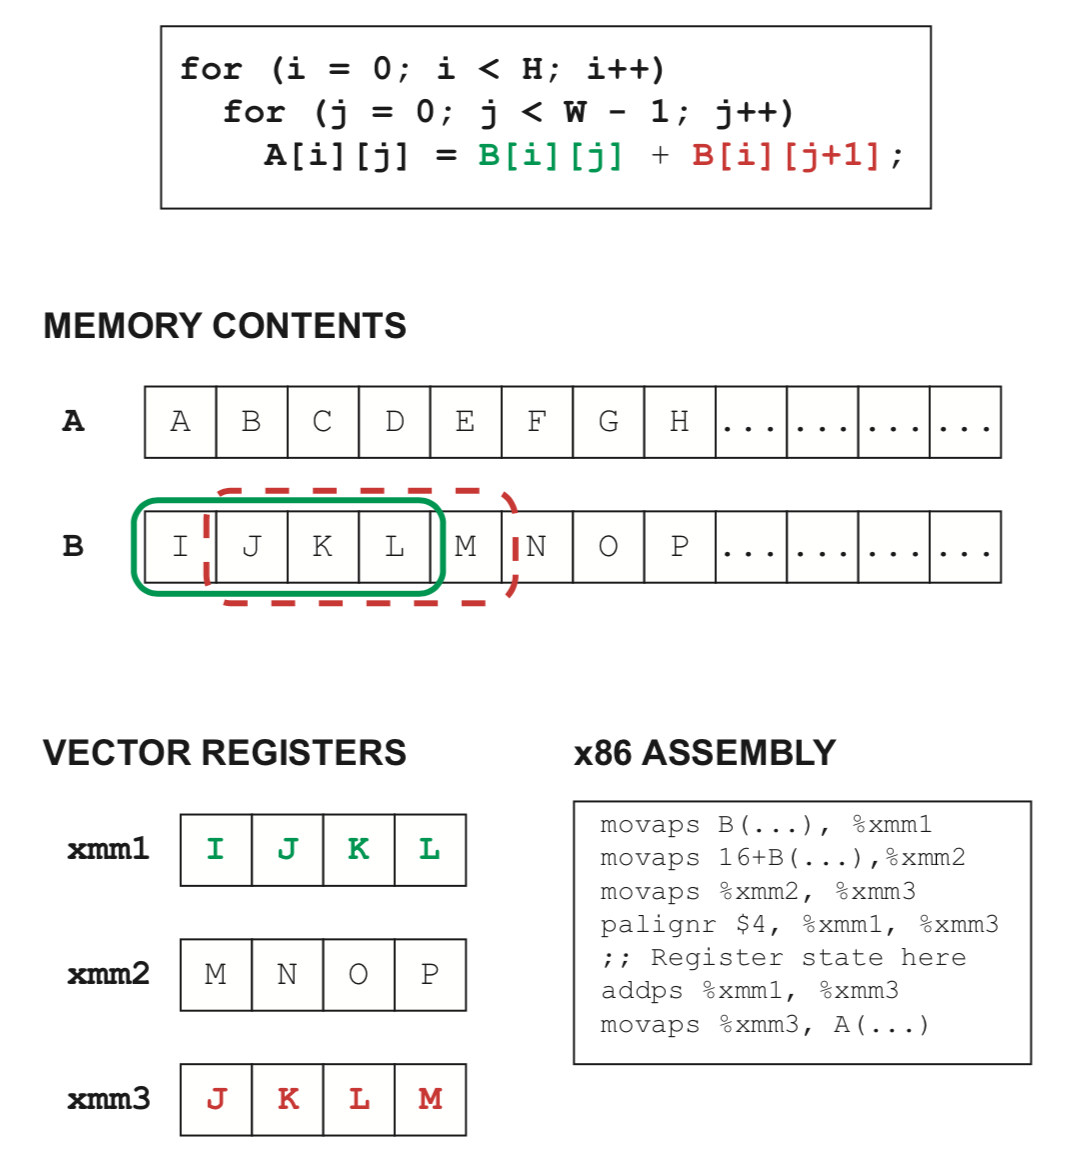
\includegraphics[height=0.85\textheight]{07/stencil-bad}}

    \only<1>{\scriptsize
      From \emph{Data Layout Transformation for Stencil Computations on
        Short-Vector SIMD Architectures} (2011)
      \url{https://web.cs.ucla.edu/~pouchet/doc/cc-article.11.pdf},
      doi:10.1007/978-3-642-19861-8\_13
    }
  \end{center}
\end{frame}

\begin{frame}[fragile]
  \frametitle{A helpful observation}
  \begin{itemize}
  \item Empirically, most code executes a small number of ``hotspots''
    that access data over-and-over.
  \item In stencil codes this might often be an ``outer'' loop
    ``time'' or similar
  \item Therefore can be worthwhile performing a \emph{data layout
      transformation} beforehand.
  \item Sometimes this can be done statically, sometimes only
    dynamically (if other parts of the program want data in a
    different format).
  \end{itemize}
\begin{minted}[fontsize=\scriptsize]{c}
while (t < T) {
  for (i = 0; i < n; i++) {
    for (j = 0; j < n; j++) {
      b[i, j] = a[i-1, j] + a[i+1, j] + a[i, j-1] + a[i, j+1] - 4*a[i, j];
    }
  }
}
\end{minted}
\end{frame}

\begin{frame}
  \frametitle{Plan}
  \begin{itemize}
  \item Two cases
    \begin{enumerate}
    \item Single access pattern in program
    \item Multiple access patterns in program
    \end{enumerate}
  \item One solution
    \begin{itemize}  
    \item Look for \emph{transformation} of data layout that gives
      better cache utilisation and vectorisation opportunities
    \end{itemize}
  \item At one of two different times
    \begin{enumerate}
    \item Single access pattern $\Rightarrow$ compile-time (static)
      layout transformation
    \item Multiple access patterns $\Rightarrow$ run-time (dynamic)
      layout transformation
    \end{enumerate}
  \item Latter case has a cost that is \emph{amortized} over the
    subsequent accesses.
  \end{itemize}
\end{frame}

\begin{frame}
  \frametitle{Vectorising on ``streams''}
  \begin{itemize}
  \item Need successive statements to have same access pattern (may be
    shifted) for vectorisation.
  \end{itemize}
  \begin{center}
    \only<1>{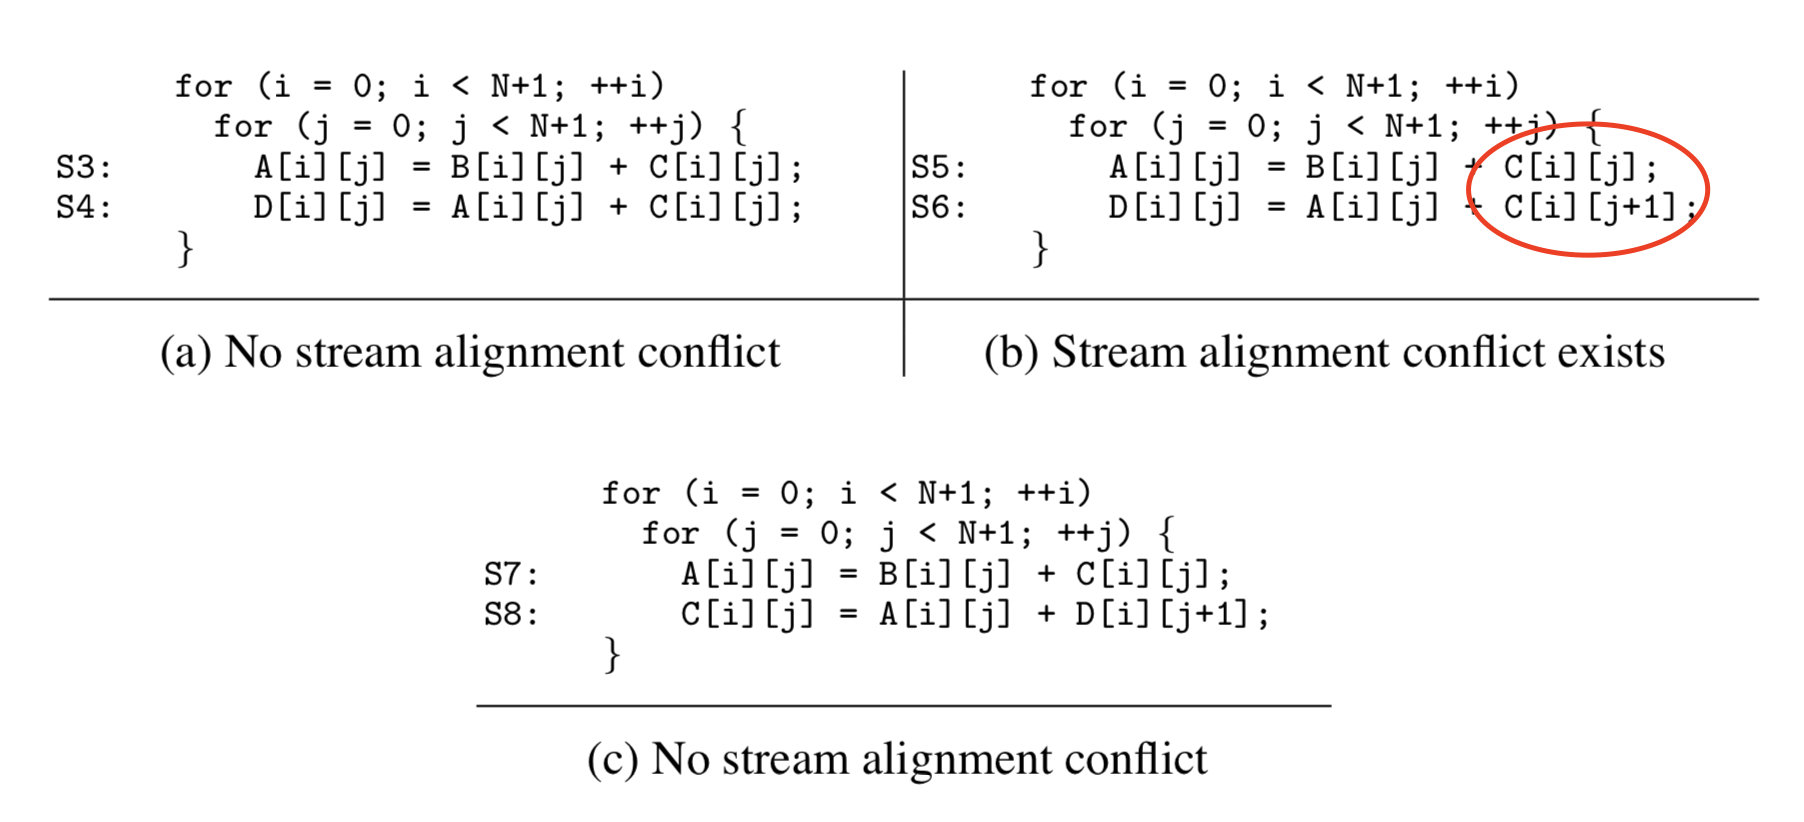
\includegraphics[height=0.6\textheight]{07/stream-alignment}}
    \only<2>{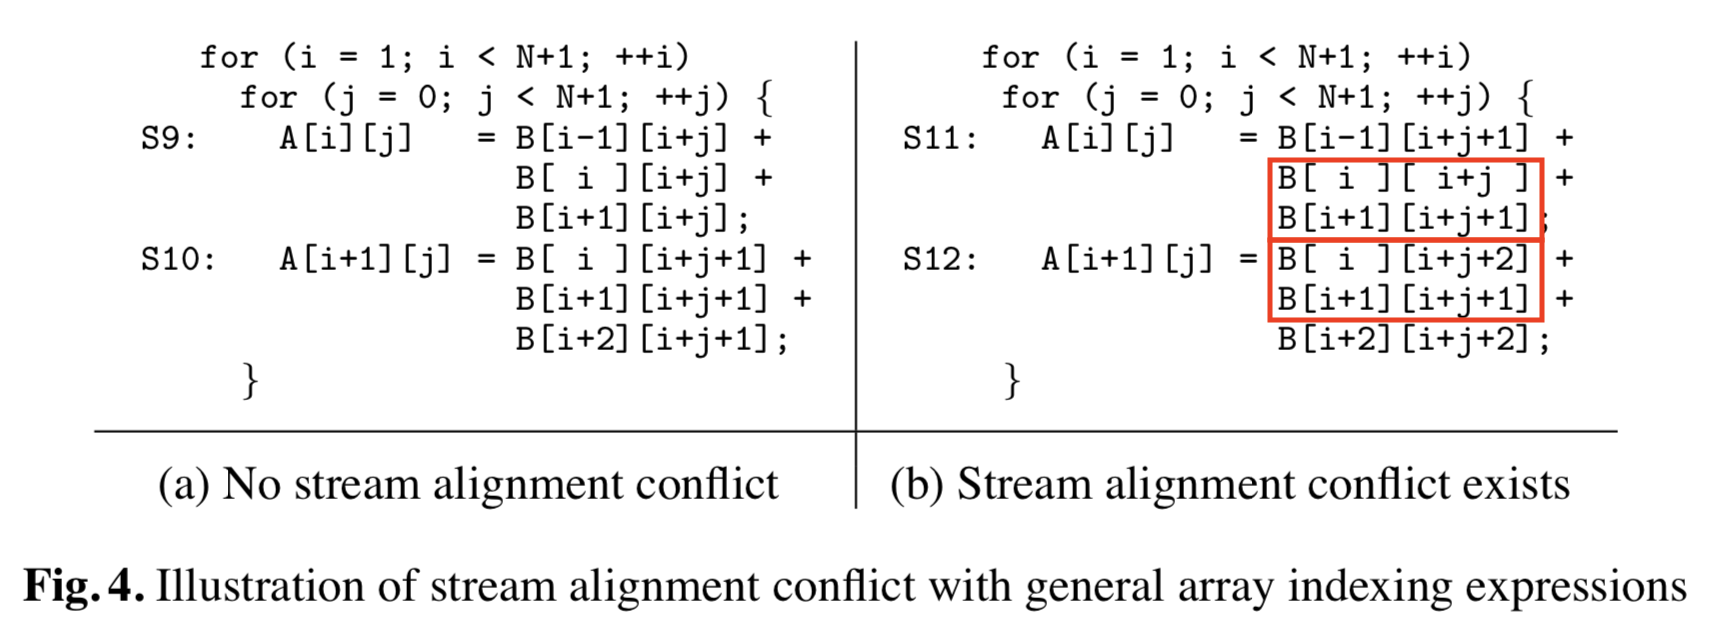
\includegraphics[width=\textwidth]{07/stream-expressions}}
  \end{center}
\end{frame}

\begin{frame}
  \frametitle{Data layout transformation}
  \only<1>{\begin{challenge}{Problem}
    \begin{itemize}
    \item Adjacent elements in memory map to adjacent slots (or lanes)
      in the vector registers.
    \item Vector operations on these adjacent elements therefore
      require more memory movement, or shuffling in registers.
    \end{itemize}
  \end{challenge}
  }

  \only<2>{\begin{answer}{Solution}
    \begin{itemize}
    \item \emph{relocate} adjacent elements \emph{such that} they can
      map to the same vector lane.
    \end{itemize}

    \begin{columns}
      \begin{column}{0.4\textwidth}
        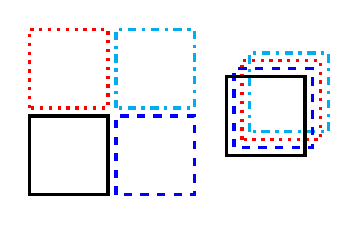
\begin{tikzpicture}
          \draw[very thick, black] (0, 0) rectangle +(1, 1);
          \draw[very thick, dashed, blue] (1.1, 0) rectangle +(1, 1);
          \draw[very thick, dotted, red] (0, 1.1) rectangle +(1, 1);
          \draw[very thick, dash dot, cyan] (1.1, 1.1) rectangle +(1,
          1);

          \draw[very thick, dash dot, cyan] (2.8, 0.8) rectangle +(1,
          1); \draw[very thick, dotted, red] (2.7, 0.7) rectangle +(1,
          1); \draw[very thick, dashed, blue] (2.6, 0.6) rectangle
          +(1, 1); \draw[very thick, black] (2.5, 0.5) rectangle +(1,
          1);
        \end{tikzpicture}
      \end{column}
      \begin{column}{0.5\textwidth}
        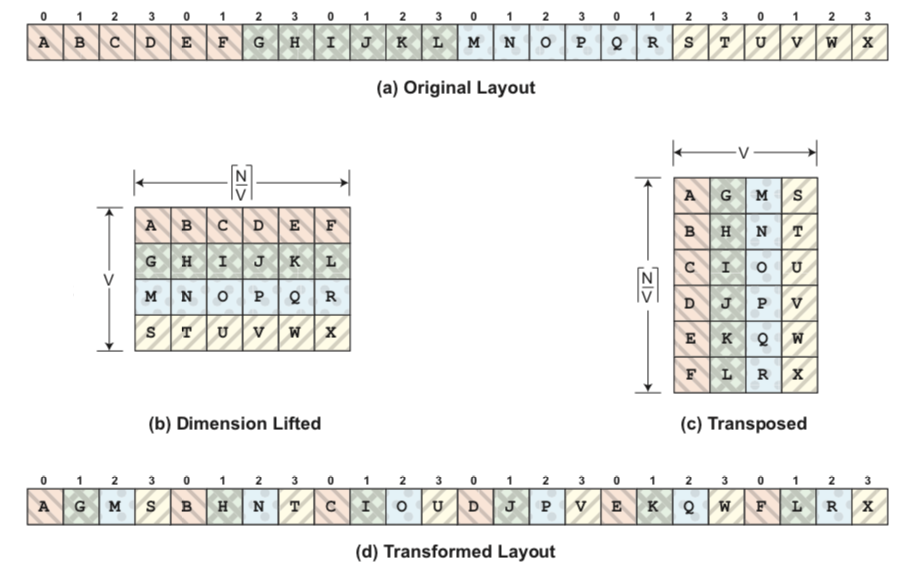
\includegraphics[width=\textwidth]{07/1d-transpose}
      \end{column}
    \end{columns}
  \end{answer}
  }
\end{frame}

\begin{frame}[fragile]
  \frametitle{With code}

  \begin{columns}
    \begin{column}{0.4\textwidth}
\begin{minted}[fontsize=\scriptsize]{c}
for (i = 0; i < 24; i++)
  Z[i] = Y[i-1] + Y[i] + Y[i+1];
\end{minted}
    \end{column}
    \begin{column}{0.6\textwidth}
\begin{minted}[fontsize=\scriptsize]{c}
for (i = 0; i < 6; i++)
  for (j = 0; j < 4; j++)
     Zt[i, j] = Yt[i-1, j] + Y[i, j] + Y[i+1, j];
\end{minted}
    \end{column}
  \end{columns}
  \begin{center}
    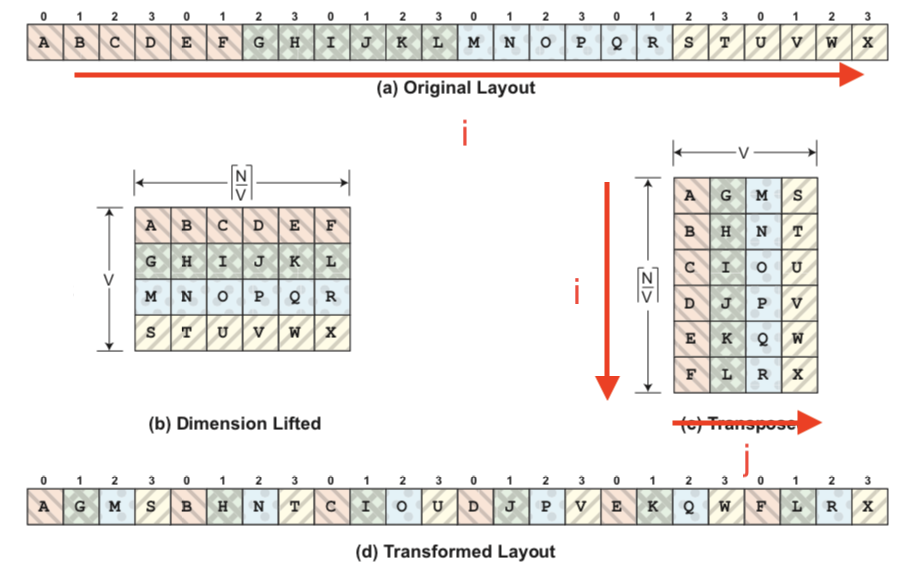
\includegraphics[width=0.6\textwidth]{07/1d-transpose-annotate}
  \end{center}
\end{frame}

\begin{frame}
  \frametitle{Same idea in higher dimensions}
  \begin{center}
    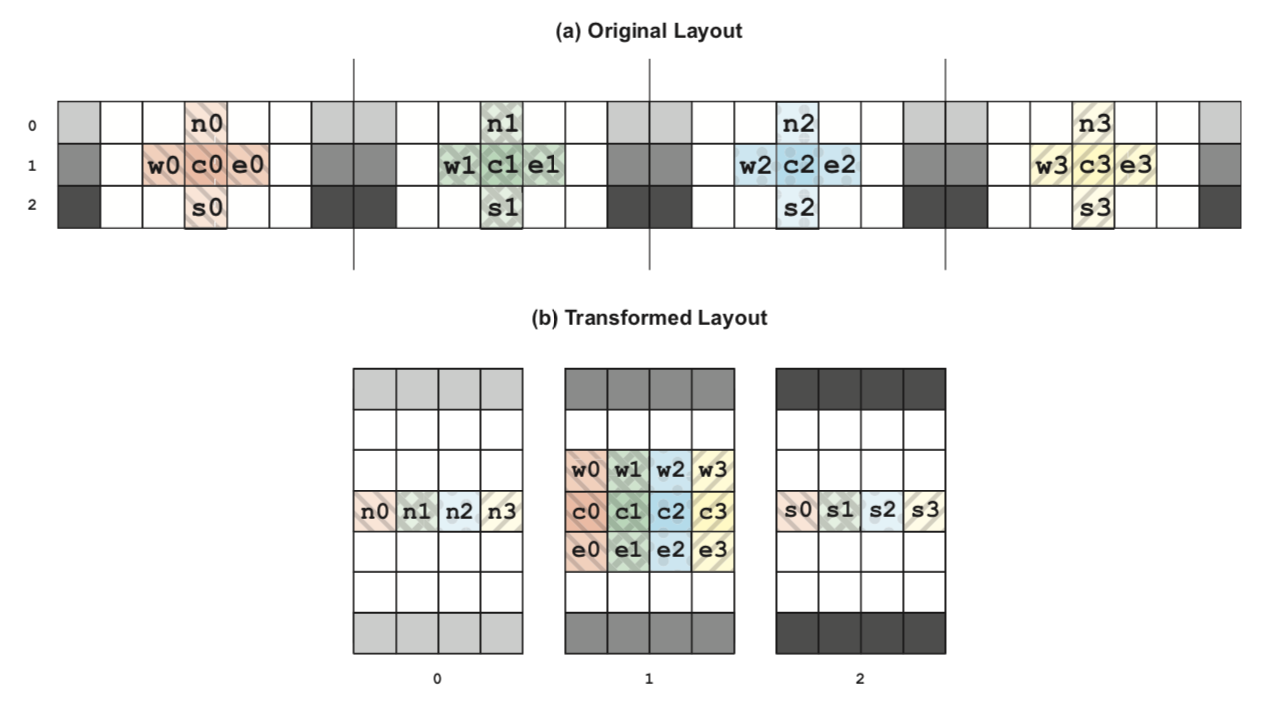
\includegraphics[width=\textwidth]{07/2d-transpose}
  \end{center}
\end{frame}

\begin{frame}
  \frametitle{What about the boundaries?}
  \only<1>{\begin{challenge}{Problem}
      \begin{itemize}
      \item This scheme works perfectly in the bulk of the domain
      \item At the edges, it is a little trickier.
      \item[$\Rightarrow$] We need to add $F + G + H$, not $F + A + B$.
      \end{itemize}
      \begin{center}
        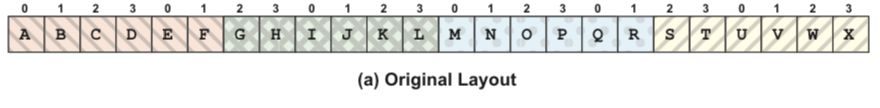
\includegraphics[width=0.9\textwidth]{07/1d-transpose-orig}

        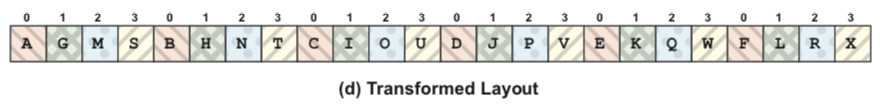
\includegraphics[width=0.9\textwidth]{07/1d-transpose-transformed}

        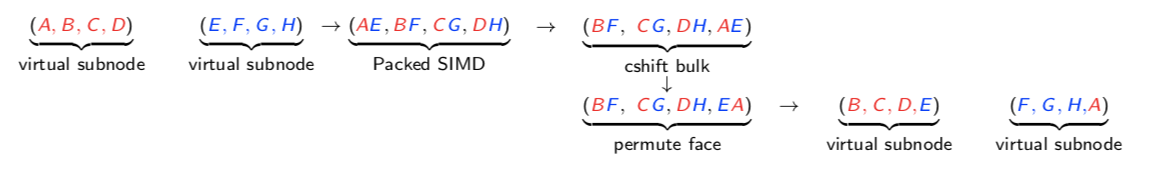
\includegraphics[width=0.9\textwidth]{07/boundaries-other}
      \end{center}
    \end{challenge}
  }
  \only<2>{
    \begin{answer}{Solution}
      \begin{itemize}
      \item Use \emph{vector shuffles} and masking to handle (literal)
        edge cases.
      \item Performance for these updates is \emph{lower} but suppressed by
        surface-to-volume ratio.
      \end{itemize}
      \begin{center}
        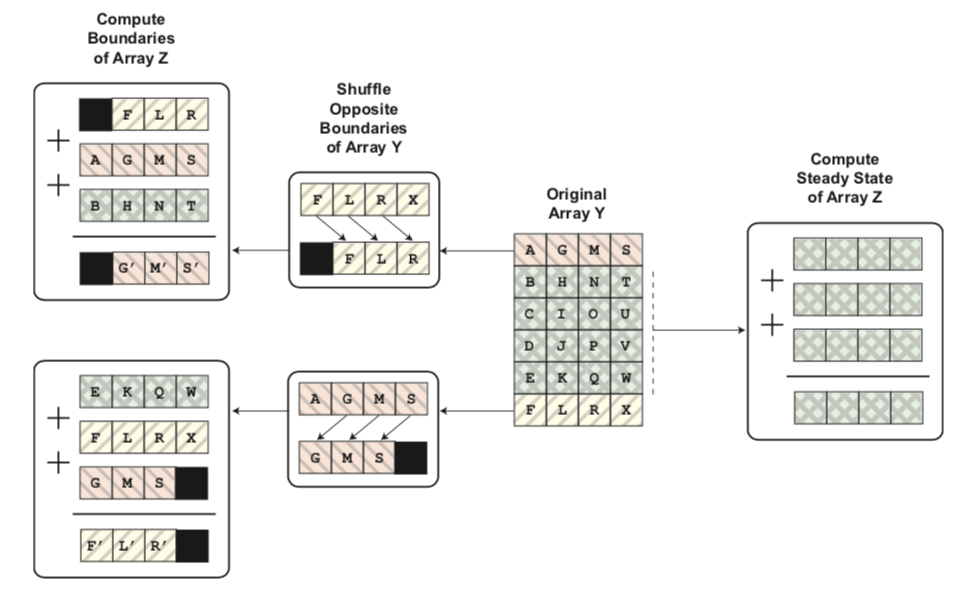
\includegraphics[width=0.6\textwidth]{07/boundaries}
      \end{center}
    \end{answer}
  }
\end{frame}

\begin{frame}[fragile]
  \frametitle{AoS vs.~SoA}
  \begin{quote}
    Use struct of arrays, not array of structs for data layout

    (NVidia)
  \end{quote}
  \begin{itemize}
  \item Why? ``Coalesced memory access''
  \item[$\Leftrightarrow$] adjacent threads access adjacent memory
    addresses
  \item Same principle applies for vectorisation
  \end{itemize}

  \begin{columns}
    \begin{column}{0.5\textwidth}
      Array of structs
      
\begin{minted}[fontsize=\scriptsize]{c}
struct Point {
  double x, y, z;
};

struct Point *points = ...;
\end{minted}
    \end{column}

    \begin{column}{0.5\textwidth}
      Struct of arrays

\begin{minted}[fontsize=\scriptsize]{c}
struct Points {
  double *x, *y, *z;
};

struct Points points = ...;
\end{minted}
    \end{column}
  \end{columns}
\end{frame}

\begin{frame}
  \frametitle{Pros and cons}
  \begin{columns}
    \begin{column}{0.5\textwidth}
      \begin{block}{AoS}
        \begin{itemize}
        \item[\cmark] most obvious (each record has all its fields
          together)
        \item[\cmark] good cache usage for streaming access to all
          fields
        \item[\cmark] Minimal memory footprint (e.g.~need one cache line for each 3D point)
        \item[\xmark] bad for vectorising (unless \# fields matches
          vector width), since natural inner loop is over fields.
        \end{itemize}
      \end{block}
    \end{column}
    \begin{column}{0.5\textwidth}
      \begin{block}{SoA}
        \begin{itemize}
        \item[\xmark] data structure a little harder to manage
        \item[\cmark] good cache usage for streaming access to each
          field
        \item[\xmark] higher memory pressure for accessing all fields
          (e.g.~need three cache lines for each 3D point)
        \item[\cmark] good for vectorising, since natural inner loop
          is over data items.
        \end{itemize}
      \end{block}
    \end{column}
  \end{columns}
\end{frame}

\begin{frame}[fragile]
  \frametitle{Best of both worlds}
  \begin{itemize}
  \item Dimension-lifted transposition ticks all boxes (presuming your
    cache is big enough).
  \item Can apply to AoS vs.~SoA argument by instead having AoSoA
    (Array of struct of (short) arrays)
  \item[$\Rightarrow$] add extra dimension to data layout and
    transpose the data.
  \end{itemize}
\begin{minted}[fontsize=\scriptsize]{c}
#define N 4 /* vector width */
struct pointN {
  double x[N], y[N], z[N];
}

struct pointN *points = ...;
\end{minted}
\end{frame}

\begin{frame}
  \frametitle{Evaluation of performance}
  \begin{center}
    \only<1>{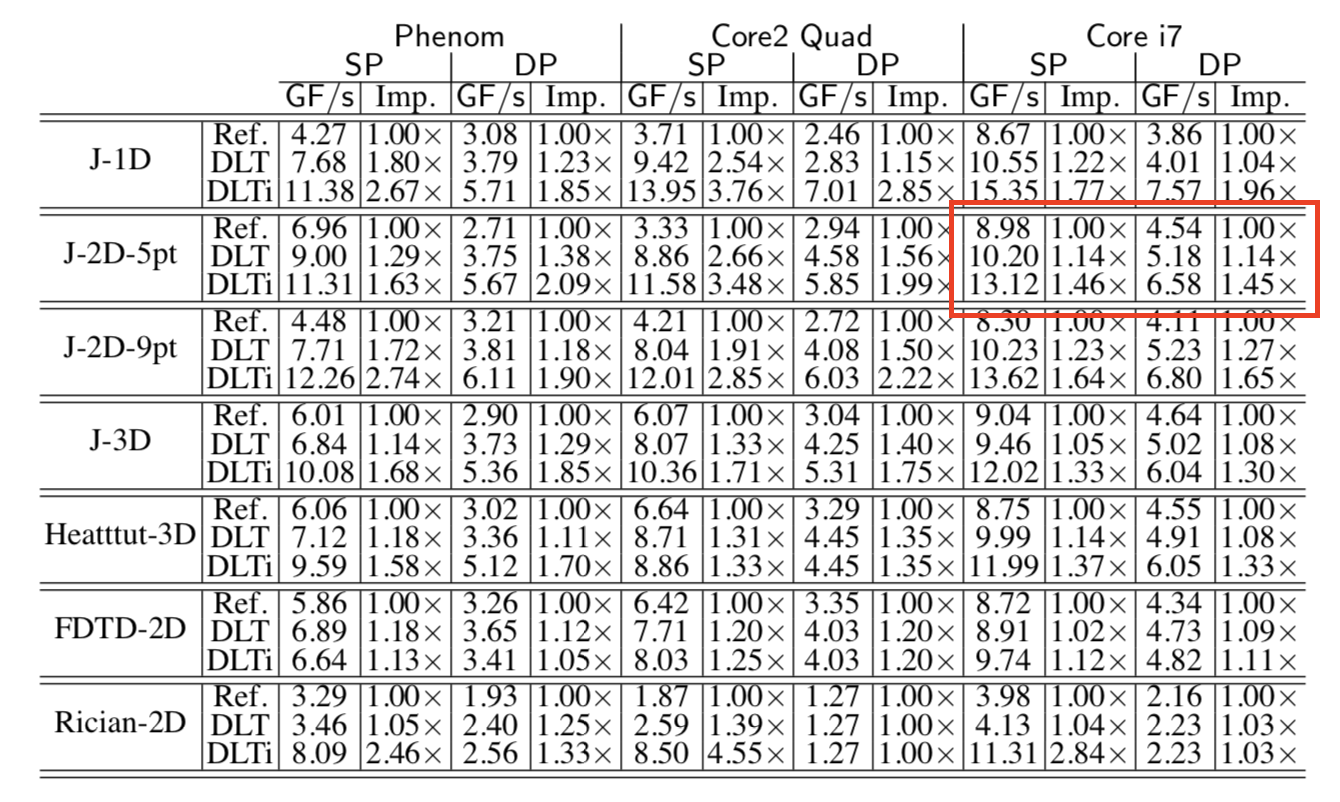
\includegraphics[width=\textwidth]{07/dlt-results}}
    \only<2>{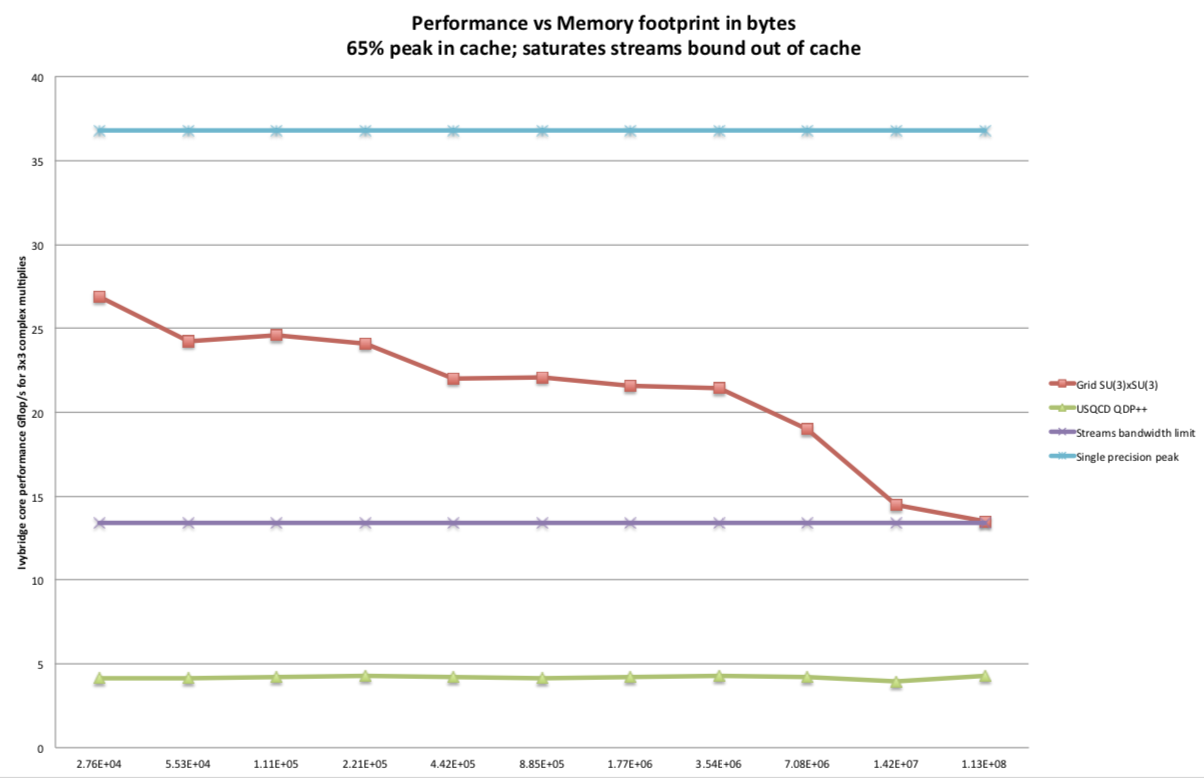
\includegraphics[width=\textwidth]{07/grid-results}}
  \end{center}
\end{frame}


\begin{frame}
  \frametitle{Summary}
  \begin{itemize}
  \item For regular (stencil-like) array access patterns, can obtain
    basically perfect cache usage and vectorisation through data
    layout transformations.
  \item Approach of ``dimension-lifting'' is generic
    \begin{itemize}
    \item Applies on both CPUs and GPUs (just use different inner
      dimension lengths)
    \item Exact details of loop structure not hugely important
    \end{itemize}
  \item Same ideas can also be applied to \emph{unstructured}
    computations with local stencils
  \end{itemize}
\end{frame}

\end{document}
